\cnote{Add the DK16 framework?}

%%%%%%%%%%%%%%%%%%%%%%%%%%%%%%%%%%%%%%%%%%%%%%%%%%%
\section{Ingster's method}
%%%%%%%%%%%%%%%%%%%%%%%%%%%%%%%%%%%%%%%%%%%%%%%%%%%
\section{Indistinguishability via moment-matching}

We will here describe a general, out-of-the-box theorem which applies to a broad class of distribution properties: namely, the class of \emph{symmetric properties}, which are those which do not depend on the individual labels of the domain elements.
\begin{definition}
	A property $\property=\cup_{\ab=1}^\infty \property_\ab$ of distributions is said to be \emph{symmetric} if it is closed under permutations of the domain: for every $\ab$ and every permutation $\sigma\colon\domain_\ab\to \domain_\ab$, if $\p\in\property_\ab$ then $\p\circ\sigma\in\property_\ab$.
\end{definition}
A by now familiar example of symmetric property is uniformity, $\property_\ab =\{\uniformOn{\ab}\}$, since the uniform distribution is invariant by relabeling: $\uniformOn{\ab}(\sigma(i))=\uniformOn{\ab}(i)$ for every $i\in\domain_\ab$ and every permutation $\sigma$ of $\domain_\ab$. Other notable examples include the property of ``all distributions of support size at most $s$,'' that of ``distributions of (Shannon) entropy at least $h$,'' but, for instance, \emph{not} the property of ``distributions with a non-increasing pmf'' (since it depends on the ordering of the domain).

The definition of symmetric properties can be extended to multiple distributions over the same domain: for instance, taking $\domain_\ab=[\ab]\times[\ab]$, a property $\property_\ab$ of product distributions is symmetric if $\p_1\otimes \p_2\in \property_\ab$ implies $\p_1\circ\sigma\otimes \p_2\circ\sigma\in \property_\ab$ for all permutations $\sigma$. This is the case, \eg of the property corresponding to {closeness testing}, $\setOfSuchThat{\p_1\otimes\p_2}{\p_1=\p_2}$, mentioned in~\cref{chap:what}.

Symmetric properties are nice in the sense that, when considering them, one can completely forget about the individual values of the $\ns$ samples taken, and focus instead on the empirical histogram. That is, a sufficient statistic for symmetric properties is the \emph{fingerprint} of the samples, which is just the tuple
\[
	\freq\eqdef (\freq_{0},\freq_{1},\freq_{2},\dots,\freq_{\ns}) \in \N^{\ns+1}
\]
where $\freq{j} = \sum_{i=1}^\ab \indic{\occur_{i}=j}$ is the number of elements of the domain which appear exactly $j$ times among the $\ns$ samples. In particular, we always have $\sum_{j=0}^\ns \freq_j = \ns$.\exercise{Check that you can express several (FOCUS ON A COUPLE) \tbc of the algorithms in~\cref{sec:uniformity} as a function of $\freq$ only.}\medskip

The main result discussed in this section is the ``Wishful Thinking Theorem'' of~\citet{Valiant:11}, which applies to testing symmetric properties of distributions. Intuitively, this theorem ensures that ``if the low-degree moments ($\lp[p]$ norms) of two distributions match, then these distributions (up to relabeling) are hard to distinguish.'' To see why this is the case, and justify the name of the theorem, observe that since we focus on symmetric properties all which matters is the fingerprint $\freq$ introduced about; that is, the number of $j$-collisions, for every $j\geq 0$.

Now, given a distribution $\p$, the number of $j$-collisions in $\ns$ samples has expectation 
\[
	\binom{\ns}{j}\norm{\p}_j^j \asymp \ns^j\norm{\p}_j^j
\]
and variance, wishfully ignoring all dependencies, maybe something like $\ns^j\norm{\p}_j^j$ as well (roughly what it would be if $j$-wise collisions were Binomial with parameters $\binom{\ns}{j}$ and $\norm{\p}_j^j$~--~again, wishful thinking). So, given two probability distributions $\p^\yes,\p^\no$, if the squared gap between the expected numbers of $j$-wise collisions was much smaller than the maximum of the two variances
\[
		(\ns^j\norm{\p^\yes}_j^j - \ns^j\norm{\p^\no}_j^j )^2 \ll
		\max(\ns^j\norm{\p^\yes}_j^j, \ns^j\norm{\p^\no}_j^j)
\]
for all $j\geq 1$; or, equivalently, 
\[
	\frac{|\ns^j\norm{\p^\yes}_j^j - \ns^j\norm{\p^\no}_j^j|}{\sqrt{\max(\ns^j\norm{\p^\yes}_j^j, \ns^j\norm{\p^\no}_j^j)}} \ll 1
\] 
for all $j\geq 1$, then we could \emph{hope} that the two distributions are indistinguishable from their fingerprints on $\ns$ samples. Well, the reasoning above is flawed in a few ways, but can be made rigorous with enough work; and, luckily, someone else took care of this already:
\begin{theorem}[Wishful Thinking Theorem {\citep[Theorem 4.10]{Valiant:11}}]\label{theo:valiant:wishful}
  Fix any \emph{symmetric} property $\property$. Given a positive integer $\ns$, a distance parameter $\dst\in(0,1]$, and two distributions $\p^\yes,\p^\no\in\distribs{\ab}$, suppose the following conditions hold:
  \begin{enumerate}
    \item $\norminf{\p^\yes},\norminf{\p^\no} \leq \frac{1}{500\ns}$;
    \item letting $m^\yes$, $m^\no$ be the $\ns$-based moments of $\p^\yes,\p^\no$ (defined below),
      \[
         \sum_{j=2}^\infty \frac{\abs{m^{\yes}(j)-m^{\no}(j)}}{\flr{j/2}!\sqrt{1+\max(m^{\yes}(j),m^{\no}(j))}} < \frac{1}{24},
      \]
      where $m^{\yes}(j) \eqdef \ns^j\norm{\p^\yes}_j^j$, $m^{\no}(j) \eqdef \ns^j\norm{\p^\no}_j^j$ for $j\geq 0$,
     \item $\p^\yes\in\property_\ab$ and $\totalvardist{\p^\no}{\property_\ab}>\dst$.
  \end{enumerate}
  Then every testing algorithm for $\property_\ab$ must have sample complexity $\ns(\ab,\dst, 1/3) > \ns$.
\end{theorem}
\noindent (Side remark: the term $j=1$ does not appear in the sum, since $\ns\norm{\p}_1=\ns$ for every distribution $\p$, and so this term always cancels out.)\medskip
%\noindent (We observe that we only reproduced here one of the three sufficient conditions given in the original, more general theorem; as this will be the only one we need.)

To see the strength of this theorem , let us use it to prove the $\bigOmega{\sqrt{\ab}/\dst^2}$ lower bound for uniformity testing. Our distribution $\p^\yes$ will, of course, have to be the uniform distribution $\uniform_\ab$ itself; as for $\p^{\no}$, let us take it to be any of the instances of ``Paninski construction'' (\cref{eq:paninski:construction}), so that
\[
	\p^{\no}(2i) = \frac{1+3\dst}{\ab}, \qquad \p^{\no}(2i-1) = \frac{1-3\dst}{\ab}, \qquad 1\leq i\leq \ab/2
\]
(where we again assume without loss of generality that $\ab$ is even, and $\dst\in(0,1/3]$). We then have 
$\totalvardist{\p^\no}{\property_\ab}=\totalvardist{\p^\no}{\uniform_\ab}= \frac{3}{2}\dst > \dst$; so let's check the two conditions of the theorem hold. 

The first condition, 
$\norminf{\p^\yes},\norminf{\p^\no} \leq \frac{1}{500\ns}$
will be satisfied as long as $\ns \leq \frac{\ab}{1000}$, since $\norminf{\p^\yes}\leq \norminf{\p^\no} \leq 2/\ab$. This is a limitation which will limit the range of applicability of the lower bound, but we can live with it (and will get back to it later).

Turning to the second condition, we need to compute these $\ns$-based moments. Luckily, it is a simple matter to check that, for every $j\geq 2$,
\begin{equation}
	\label{eq:moments:yes}
	m^{\yes}(j) = \frac{\ns^j}{\ab^{j-1}}
\end{equation}
while
\begin{align}
	m^{\no}(j) 
	&= \ns^j \sum_{i=1}^\ab \p^{\no}(i)^j 
	= \ns^j\Paren{ \frac{\ab}{2} \Paren{\frac{1+3\dst}{\ab}}^j + \frac{\ab}{2} \Paren{\frac{1-3\dst}{\ab}}^j } \notag\\
	&= \frac{\ns^j}{\ab^{j-1}}\Paren{ \frac{(1+3\dst)^j + (1-3\dst)^j}{2} }
	\leq \frac{2^j\ns^j}{\ab^{j-1}} \label{eq:moments:no}
\end{align}
For instance, for the special case of $j=2$, the expression is a little nicer, and becomes
\begin{equation}
	m^{\no}(2)
	= (1+9\dst^2)\frac{\ns^2}{\ab}\,.
\end{equation}
Without wanting to spoil the surprise, we ``should'' expect the term $j=2$ of the series $\sum_{j=2}^\infty \frac{\abs{m^{\yes}(j)-m^{\no}(j)}}{\flr{j/2}!\sqrt{1+\max(m^{\yes}(j),m^{\no}(j))}}$ to dominate (as the second moment $\normtwo{\p}^2$ of the distribution is ``what gives it away'' in uniformity testing, as we saw now and again in~\cref{sec:uniformity}), so we will want to make sure we handle that term as tightly as possible.\medskip

With the above expressions at our disposal, we can proceed: first, since the series decays quite fast already (at least geometrically) as $\ns/\ab \ll 1$, the factorial in the denominator does not look crucial and it seems reasonable to ignore it. Moreover this maximum in the denominator seems annoying and will prevent us from easily computing the series, so let's get rid of it as well:
\begin{align*}
\sum_{j=2}^\infty \frac{\abs{m^{\yes}(j)-m^{\no}(j)}}{\sqrt{1+\max(m^{\yes}(j),m^{\no}(j))}}
&\leq
\sum_{j=2}^\infty \abs{m^{\yes}(j)-m^{\no}(j)} \\
&\leq \frac{9\dst^2\ns^2}{\ab} + \sum_{j=3}^\infty \frac{(2^j-1)\ns^j}{\ab^{j-1}} \\
&\leq \frac{9\dst^2\ns^2}{\ab} + 2\ns\sum_{j=2}^\infty \frac{2^j\ns^j}{\ab^{j}} \\
&= \frac{9\dst^2\ns^2}{\ab} + \frac{8\ns^3}{\ab^2}\cdot \frac{1}{1-2\ns/\ab} \\
&\leq \frac{9\dst^2\ns^2}{\ab} + \frac{9\ns^3}{\ab^2}
\end{align*}
where we used the assumption that $\ns\leq \ab/1000$ to guarantee convergence of the geometric series, and bound its sum. Now, even ignoring the second term, we see that the RHS will only be less that $1/24$ (as required by the second condition of the theorem) if $\ns \ll \sqrt{\ab}/\dst$, so the best lower bound we can hope for is $\bigOmega{\sqrt{\ab}/\dst}$. But we wanted $\bigOmega{\sqrt{\ab}/\dst^2}$!\smallskip

\noindent Oops.\smallskip

\noindent What went wrong? We were a little too eager to get rid of ``this maximum in the denominator.'' It \emph{is} annoying, and it \emph{is} a good idea to get rid of it in order to be left with a geometric series (at least to get a sense of what is going on), but \emph{not} in that way. Let's try again.
\begin{align*}
\sum_{j=2}^\infty \frac{\abs{m^{\yes}(j)-m^{\no}(j)}}{\sqrt{1+\max(m^{\yes}(j),m^{\no}(j))}}
&\leq
\sum_{j=2}^\infty \frac{\abs{m^{\yes}(j)-m^{\no}(j)}}{\sqrt{m^{\yes}(j)}} \\
&= \sum_{j=2}^\infty \frac{\ns^{j/2}}{\ab^{{(j-1)/2}}}\Paren{ \frac{(1+3\dst)^j + (1-3\dst)^j}{2} - 1 } \\
&= \frac{1}{2\sqrt{\ab}}\sum_{j=2}^\infty (\alpha^j+\beta^j-2\gamma^j)
\end{align*}
where $\alpha \eqdef (1+3\dst)\sqrt{\ns/\ab}$, $\beta \eqdef (1-3\dst)\sqrt{\ns/\ab}$, $\gamma \eqdef \sqrt{\ns/\ab}$, and we used~\cref{eq:moments:yes,eq:moments:no} for the first equality. Since all three are in $(0,1)$ (recall that we have $\ns \ll \ab$), we can compute the geometric series to get
\begin{align*}
\sum_{j=2}^\infty &\frac{\abs{m^{\yes}(j)-m^{\no}(j)}}{\sqrt{1+\max(m^{\yes}(j),m^{\no}(j))}} \\
&\qquad\leq \frac{1}{2\sqrt{\ab}}\Paren{ \frac{(1+3\dst)^2\gamma^2}{1-(1+3\dst)\gamma}+\frac{(1-3\dst)^2\gamma^2}{1-(1-3\dst)\gamma}-\frac{2\gamma^2}{1-\gamma} }
\end{align*}
This looks better! Sure, this is quite ugly; but a Taylor expansion at $0$ (since $\gamma = \sqrt{\ns/\ab} \ll 1$) tells us that the parenthesis of the RHS
is
\[
	18\dst^2 \gamma^2 + o(\gamma^2) = \frac{18\dst^2\ns}{\ab} + \littleO{\frac{\ns}{\ab}}
\]
so we should be fine; and indeed, one can check that that parenthesis is equal to
\begin{align*}
%\frac{(1+3\dst)^2\gamma^2}{1-(1+3\dst)\gamma}+\frac{(1-3\dst)^2\gamma^2}{1-(1-3\dst)\gamma}-\frac{2\gamma^2}{1-\gamma} &= 
\frac{18\dst^2\gamma^2}{(1-\gamma)(1-(1+3\dst)\gamma)(1-(1-3\dst)\gamma)} \leq 144 \dst^2\gamma^2\,.
\end{align*}
From this, we get
\begin{equation}
	\sum_{j=2}^\infty \frac{\abs{m^{\yes}(j)-m^{\no}(j)}}{\sqrt{1+\max(m^{\yes}(j),m^{\no}(j))}}
	\leq \frac{1}{2\sqrt{\ab}} \cdot 144\dst^2\frac{\ns}{\ab} = \frac{72\dst^2\ns}{\sqrt{\ab}}\,.
\end{equation}
This in turn will be less than $1/24$ for $\ns \leq \sqrt{\ab}/(1728\dst^2)$. Success! Recalling finally the condition $\ns \ll \ab/$ (for the first condition of the Wishful Thinking theorem to hold) which imposes $\dst \gg 1/\ab^{1/4}$, by invoking~\cref{theo:valiant:wishful} we get the result we wanted:
\begin{theorem}
  \label{prop:uniformity:lb:valiant}
Every testing algorithm for uniformity must have sample complexity $\ns(\ab,\dst,1/3) = \Omega(\sqrt{\ab}/\dst^2)$, provided that $\dst \geq 1/\ab^{1/4}$.
\end{theorem}
The key aspect of this lower bound was how \emph{painless} it was to obtain it. The main idea was to use the same Paninski construction as before, check a couple conditions, compute a geometric series, and then conclude by~\cref{theo:valiant:wishful}. (Sure, it might have felt a \emph{little} longer than this, but this is mostly due to the author's choice of going through two consecutive attempts, instead of skipping directly to the second one.)


%%%%%%%%%%%%%%%%%%%%%%%%%%%%%%%%%%%%%%%%%%%%%%%%%%%
\section{Indistinguishability on an instance-by-instance basis}
We will now discuss and illustrate the use of a very convenient (albeit intimidating) result due to~\citet{ValiantV17}, which allows one to establish lower bounds tailored to any reference distribution $\q$.
\begin{theorem}
        \label{theo:vv:lb}
    Given a distribution $\q$ over $[\ab]$, and associated values $\alpha_i$ such that $\alpha_i \in [0,1]$ for all $i\in[\ab]$, define the set of distributions $\class=\{\p_z\}_{z\in\bool^\ab}$ by setting, for every $z\in\bool^\ab$,
\begin{equation}
	\label{eq:vv:def:hardcase}
    		\p_z(i) \eqdef \frac{(1+z_i\alpha_i)\q(i)}{\sum_{j=1}^\ab (1+z_j\alpha_j)\q(j) }, \qquad i\in[\ab]
\end{equation}
 \ie $\p_z(i) \propto (1+z_i\alpha_i)\q(i)$. 
Then there exists an absolute constant $c>0$ such that any algorithm which, given $\ns$ \iid samples from an arbitrary distribution $\p$, distinguishes with success probability at least $2/3$ between (i)~$\p=\q$ and (ii)~$\p\in\class$, must satisfy
\begin{equation}
	\label{eq:vv:lb:samples}
		\ns \geq \frac{c}{\sqrt{\sum_i \alpha_i^4\q(i)^2}}\,.
\end{equation}
Further, if $\max_{i} \alpha_i\q(i) \leq \frac{1}{2}\sum_{i=1}^\ab \alpha_i\q(i)$, then
\begin{equation}
	\label{eq:vv:proba:far}
	\bP{Z}{\totalvardist{\p_Z}{\q} > \frac{1}{4}\sum_{i=1}^\ab \alpha_i\q(i) } \geq \frac{1}{2}\,,
\end{equation}
where $Z$ is uniformly random on $\bool^\ab$.
\end{theorem}
This is a bit of a mouthful, so let's break~\cref{theo:vv:lb} down before seeing a few corollaries and applications. First, given a reference distribution $\q$, and a choice of ``element-wise perturbations'' values $\alpha_1,\dots,\alpha_\ab$,~\cref{eq:vv:def:hardcase} says we should define a ``hard instance'' by setting $\p(i) = (1\pm \alpha_i)\q(i)$, choosing the sign independently and uniformly at random for every $i$, and then normalizing the resulting $\p$ to make it a true probability distribution. After doing this,~\cref{eq:vv:lb:samples} states that distinguishing $\q$ from a hard instance $\p$ chosen randomly this way requires
$
\Omega(1/\sqrt{\sum_i \alpha_i^4\q(i)^2})
$ samples. Finally,~\cref{eq:vv:proba:far} tells us that (until some mild condition on the $\alpha_i$'s), most of those hard instances are actually \emph{far} from $\q$; in particular, we will typically want to choose the $\alpha_i$'s so that the guaranteed distance
$
\frac{1}{4}\sum_{i=1}^\ab \alpha_i\q(i)
$ is equal to our parameter $\dst$.\medskip

But \emph{how} should we choose these values $\alpha_1,\dots,\alpha_\ab$? In view of what we just discussed, it seems natural to set $\alpha_i \eqdef 4\dst$ for all $i$, ensuring that $\frac{1}{4}\sum_{i=1}^\ab \alpha_i\q(i) = \dst$. This also immediately satisfies $\max_{i} \alpha_i\q(i) \leq \frac{1}{2}\sum_{i=1}^\ab \alpha_i\q(i)$, as long as $\norminf{\q}\leq 1/2$: a rather mild condition. As for~\cref{eq:vv:lb:samples}, plugging in this choice of $\alpha_i$'s shows that it becomes
\[
		\ns \gtrsim \frac{1}{\dst^2\normtwo{\q}}
\]
which seems\dots good? For instance, when $\q$ is the uniform distribution, then $\normtwo{\q}=1/\sqrt{\ab}$, and we get an $\Omega(\sqrt{\ab}/\dst^2)$ lower bound! Specifically, we (almost) proved:
\begin{theorem}
  \label{theo:uniformity:lb:vv}
Every testing algorithm for identity with reference $\q$ must have sample complexity $\ns(\ab,\dst,1/3) = \Omega(1/(\dst^2\normtwo{\q}))$, provided that $\norminf{\q}\leq 1/2$.

In particular, every testing algorithm for uniformity must have sample complexity $\ns(\ab,\dst,1/3) = \Omega(\sqrt{\ab}/\dst^2)$.
\end{theorem}
\begin{proof}
The above discussion, combined with~\cref{theo:vv:lb}, \emph{almost} establishes the result we want, up to some annoying detail: the success probability is not exactly what we needed, due to the fact that~\cref{theo:vv:lb} only guarantees a random distribution $\p_z$ is $\dst$-far from $\q$ with probability $1/2$. Namely, assume we have a testing algorithm $\Algo$ for identity with reference $\q$ with sample complexity $\ns=\ns(\ab,\dst,1/3)$. We can use it to distinguish between $\p=\q$ and a (uniformly randomly chosen) $\p$ from $\class$ (as defined with our choice $\alpha_i = 4\dst$), giving that
(1)~if the distribution is $\q$, then we say so with probability at least $2/3$ (good);
(2)~if the distribution is $\dst$-far from $\q$, then we say $\p\in\class$ with probability at least $2/3$ (good);
\emph{but} if (3)~if the distribution is in $\class$ but \emph{not} $\dst$-far from $\q$, then we cannot say anything about being right or wrong (bad). So when $\p$ is chosen at random from $\class$, we can only guarantee we are correct with probability at least $2/3\cdot (1/2) = 1/3$\dots not $2/3$, which would be necessary to get the sample complexity lower bound from~\cref{theo:vv:lb} (\cref{eq:vv:lb:samples}) to apply.

Fortunately, there is a fix. Define $\Algo'$ as follows: given ``enough'' samples (but still $O(\ns)$), it runs $\Algo$ on disjoint subsets of $\ns$ samples and takes a majority vote, to amplify its success probability from $2/3$ to $3/4$ (as described in~\cref{lemma:error:proba:amplification}). Looking at the output, it then does the following:
\begin{itemize}
	\item if the output is $1$ ($\p\neq \q$), then it outputs $1$;
	\item if the output is $0$ ($\p=\q$), then it outputs $0$ with probability $17/24$, and $1$ with probability $7/24$.
\end{itemize}
Why did we do this? If $\p=\q$, then the probability that $\Algo'$ correctly outputs $0$ is now at least
$
\frac{3}{4}\cdot \frac{17}{24} > \frac{1}{2}
$ (worse than before). But if $\p\in\class$, it will (correctly) output $1$ with probability at least
\[
	\frac{3}{4}\cdot \frac{1}{2}+\frac{1}{2}\cdot \frac{7}{24} > \frac{1}{2}
\]
(better than before). Since both probabilities are constants greater than $1/2$, we can again use the same amplification trick (\cref{lemma:error:proba:amplification}) on $\Algo'$ to get $\Algo''$, which is correct in distinguishing $\p=\q$ from $\p\in\class$ with probability at least $2/3$ in both cases. Moreover, since all these amplications only required to blow up the sample complexity by a constant factor, $\Algo''$ still uses $\ns' = O(\ns)$ samples, and applying~\cref{theo:vv:lb} on $\Algo''$ leads to
\[
	\ns' = \Omega(1/(\dst^2\normtwo{\q}))
\]
which implies $\ns = \Omega(1/(\dst^2\normtwo{\q}))$.
\end{proof}
\exercise{Apply this to the Binomial distribution, to get $\Omega(\ab^{1/4}/\dst^2)$.}
This corollary is very handy, and provides a non-trivial lower bound as a function of some easily interpretable function of the reference $\q$. One can even generalize it to distributions over $\N$ instead of $[\ab]$ (infinite discrete domains), keeping the same statement and proof!

This raises the question: is~\cref{theo:uniformity:lb:vv} always optimal? Or, to put things more bluntly: is allowing for different $\alpha_i$'s in~\cref{theo:vv:lb} useful, or is it just for show, and unnecessarily complicated?

It is not just for show. Consider the following ``Zipf'' distribution $\q$ on $[\ab]$, where $\q(i) \propto 1/\sqrt{i}$:
\begin{equation}
	\q(i) = \frac{1}{H_{\ab,1/2} \sqrt{i}}, \qquad i \in [\ab]\,,
\end{equation}
where
\[
	H_{\ab,1/2} \eqdef \sum_{i=1}^\ab \frac{1}{\sqrt{i}} \operatorname*{\sim}_{\ab\to\infty} 2\sqrt{\ab}
\]
is the generalized Harmonic number of order $1/2$ (and $H_\ab$ will be the usual Harmonic number). A direct computation then shows that
\[
	\normtwo{\q} = \frac{\sqrt{H_\ab}}{H_{\ab,1/2}} \operatorname*{\sim}_{\ab\to\infty} \frac{\sqrt{\ln \ab}}{2\sqrt{\ab}}\,,
\]
and so~\cref{theo:uniformity:lb:vv} gives a lower bound of $\bigOmega{\frac{\sqrt{\ab}}{\dst^2\sqrt{\log \ab}}}$ samples. This does not look too bad, especially since we know from~\cref{chap:identity} that an \emph{upper} bound of  $\bigO{{\sqrt{\ab}}/{\dst^2}}$ samples holds. But that leaves a gap of $\sqrt{\log \ab}$ between the two, which could go either way.

However, let us look at this $\q$, and what a typical ``local perturbation'' $\p\in\class$ looks like when we perturb each element by $1\pm\dst$:
%%%%%%%%%%%%%%%%%%%%%%%%%%%%%%%%%%%%%%%%%%%%%%%%%%%%%%%%%%%%%%%%%%%%%%%%%
\begin{figure}[H]
	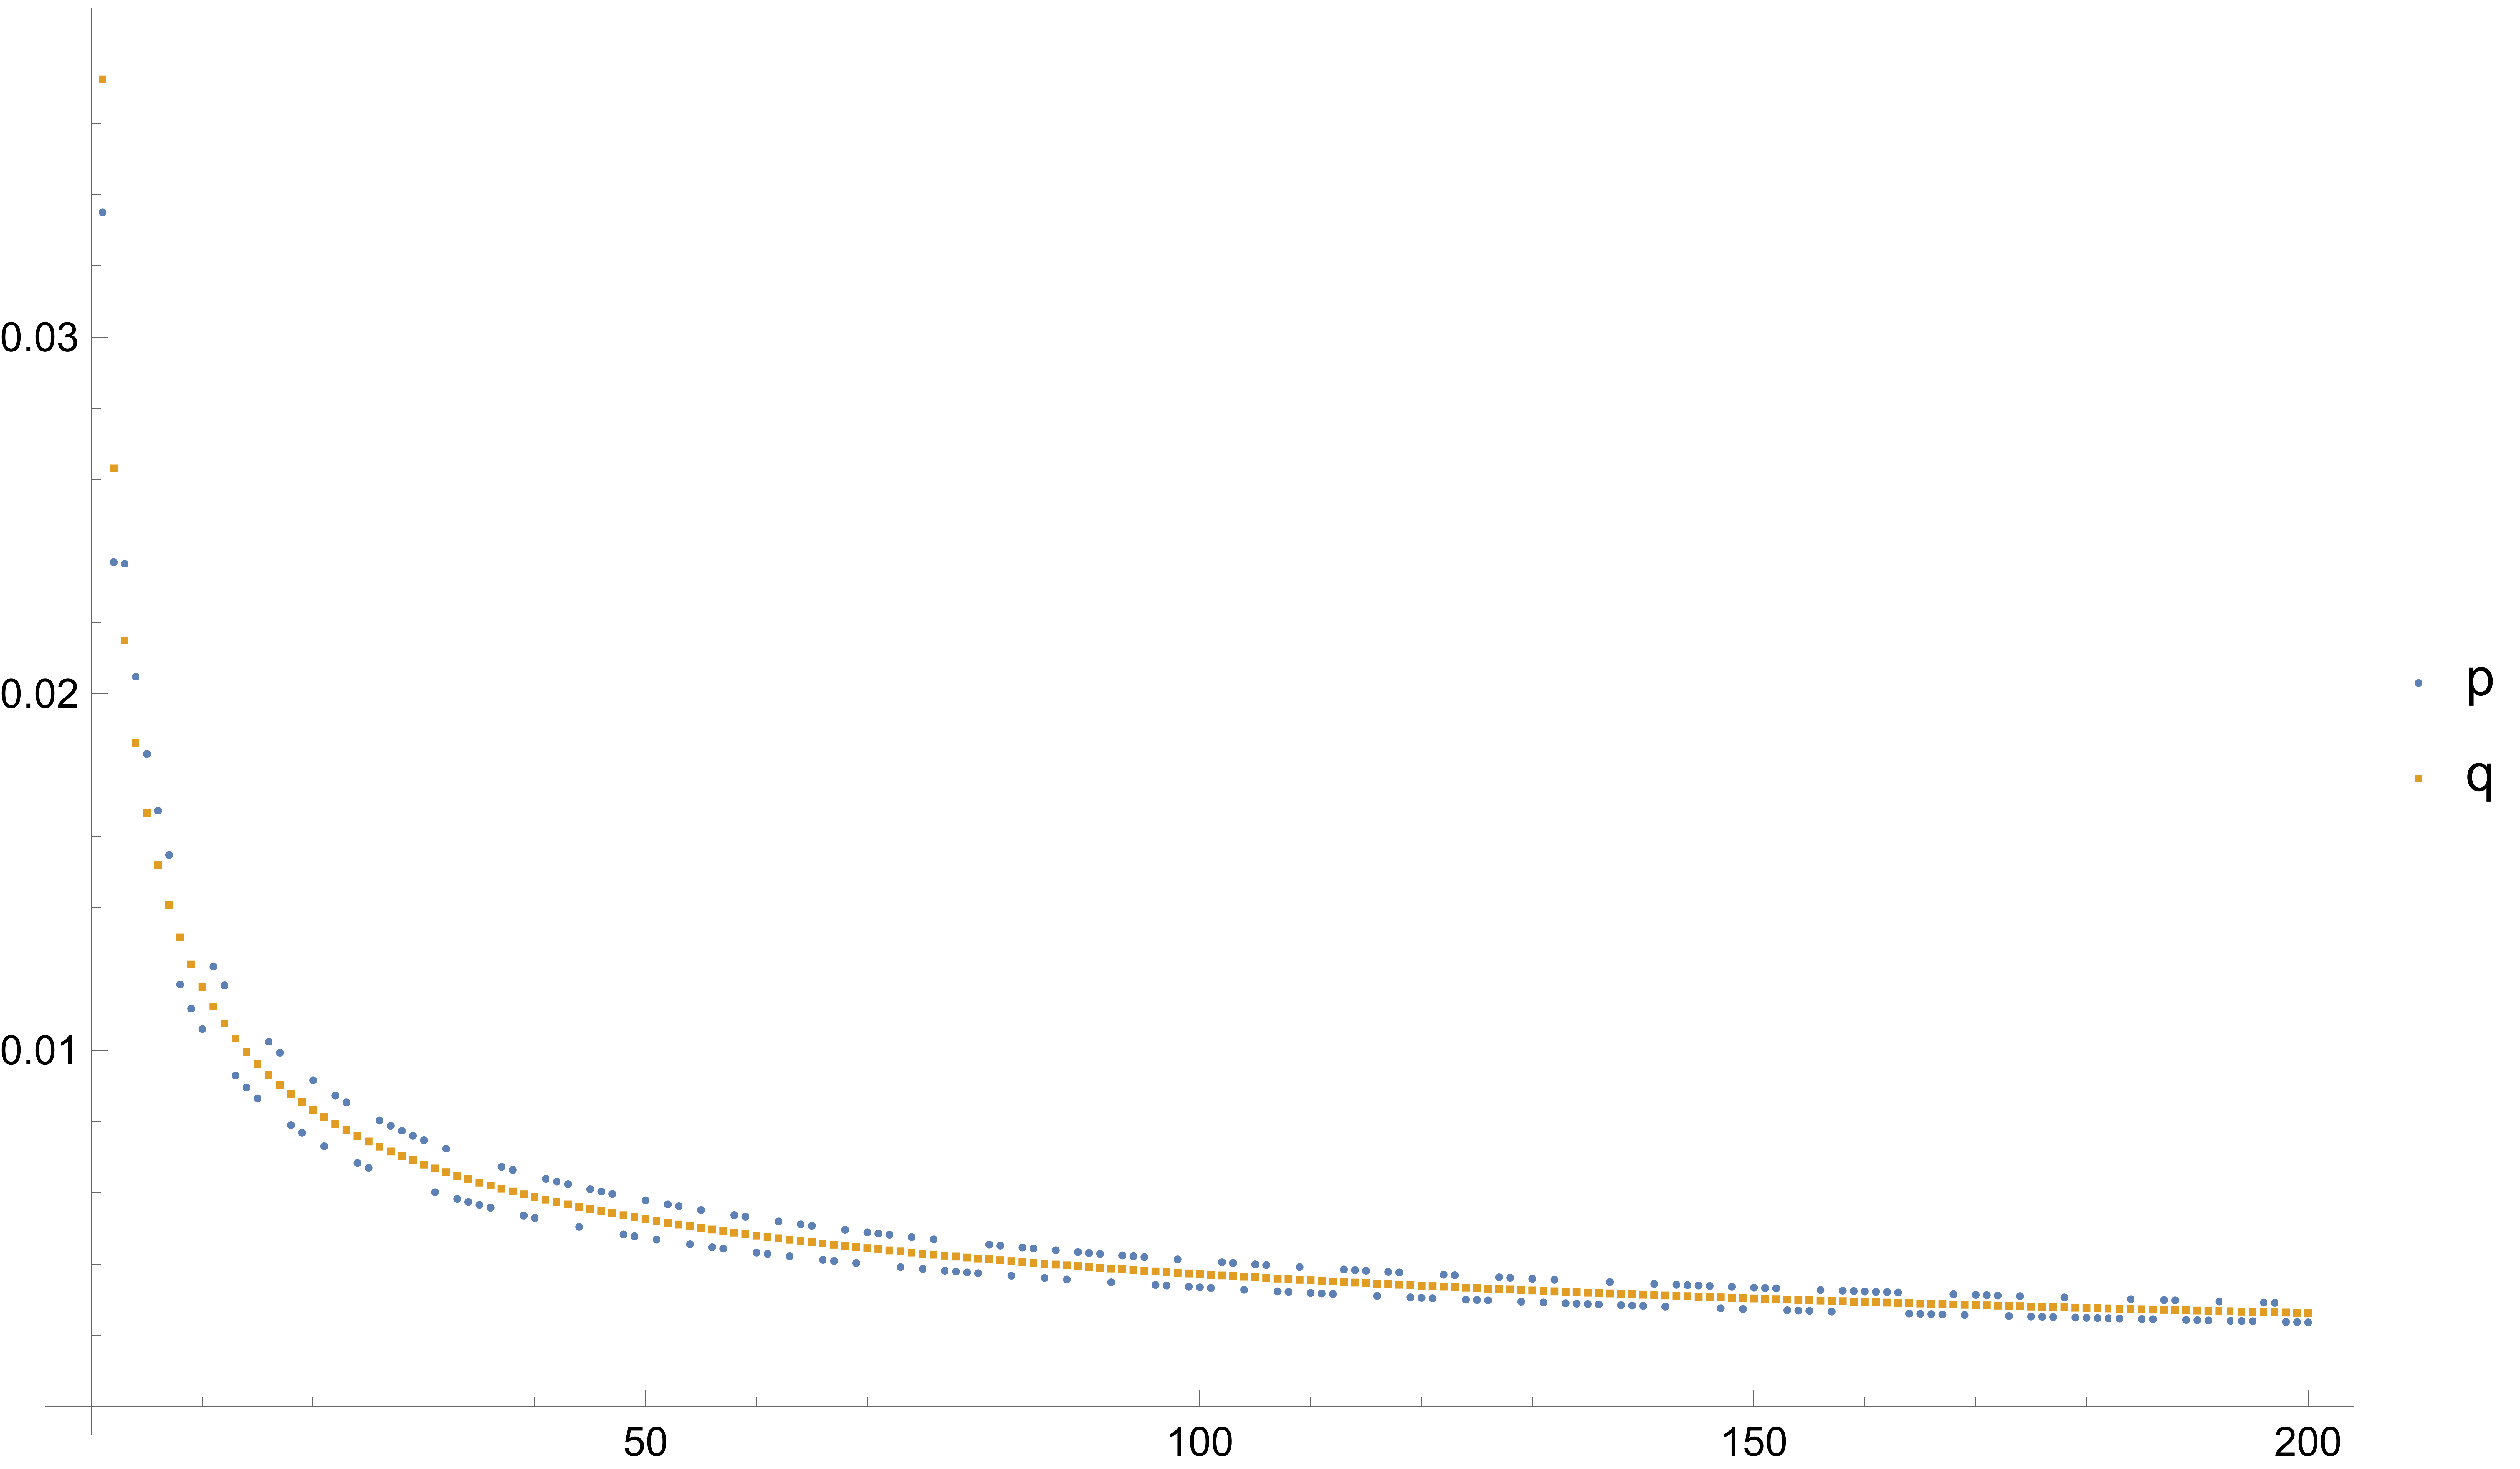
\includegraphics[width=1.0\textwidth]{figures/fig-lowerbound-zipf-pq}
	\caption{\label{fig:vv17:lb:zipf}Our reference $\q$ (Zipf distribution), along with a randomly chosen perturbation $\p$, here depicted for $\ab=200$, $\dst=1/10$.}
\end{figure}
%%%%%%%%%%%%%%%%%%%%%%%%%%%%%%%%%%%%%%%%%%%%%%%%%%%%%%%%%%%%%%%%%%%%%%%%%
While the second half (``tail'') of the distribution looks somewhat uniform (all probabilities between $\ab/2$ and $\ab$ are within a factor $\sqrt{2}$), the first half is clearly not, with the first few elements having much higher probability. Perturbing those heavy elements by the same relative amount as the rest, ``intuitively,'' is not a good idea, as it is easier to detect and can give away a lot more information. Instead, we will see what happens when we only perturb this somewhat-uniform tail of $\q$: define our $\alpha_i$'s by
\[
	\alpha_i \eqdef 
	\begin{cases}
		16\dst &\text{if } i \geq \frac{\ab}{2}\\
		0 &\text{ otherwise}
	\end{cases}
\]
In view of applying~\cref{theo:vv:lb}, we first check that the distance of our hard instances $\p_z$ to $\q$ will be at least $\dst$:
$
\max_{i} \alpha_i\q(i) = 16\dst\q(\ab/2) \ll \dst
$, and
\[
	\frac{1}{4}\sum_{i=1}^\ab \alpha_i\q(i) = 	\frac{4\dst}{H_{\ab,1/2}} \sum_{i=\frac{\ab}{2}}^\ab \frac{1}{\sqrt{i}} = 4\dst\Paren{1-\frac{H_{\frac{\ab}{2},1/2}}{H_{\ab,1/2}}} \geq 4\Paren{1-\frac{1}{\sqrt{2}}}\dst > \dst\,,
\]
so by~\cref{eq:vv:proba:far} the distance is fine. Turning to the sample complexity lower bound this will lead to, we compute
\[
	\sum_{i=1}^\ab \alpha_i^4 \q(i)^2 = \frac{(16\dst)^4}{H_{\frac{\ab}{2},1/2}^2}\sum_{i=\frac{\ab}{2}}^\ab \frac{1}{i} 
	= \frac{(16\dst)^4}{H_{\frac{\ab}{2},1/2}^2} \Paren{ H_{\ab} - H_{\frac{\ab}{2}} }
	\asymp \frac{\dst^4}{\ab}
\] 
since $H_{\ab} - H_{\ab/2} = \ln 2 + o(1)$. By~\cref{eq:vv:lb:samples}, this means we get a (tight) lower bound of $\Omega(\sqrt{\ab}/\dst^2)$ samples! All we needed to do was to restrict our perturbation to the ``near-uniform'' part of the reference distribution; crucially, this required the ability to choose different $\alpha_i$'s for different $i$, as allowed by~\cref{theo:vv:lb}.\medskip

To conclude this section, we will derive another corollary to~\cref{theo:vv:lb}, which provides the ``best'' perturbation possible for any given reference $\q$; that is, an optimal choice for the $\alpha_i$'s as a function of $\q$. Based on our previous example, we know that $\alpha_i$ somehow has to \emph{adapt} to $\q(i)$, to differentiate between the heavy elements and the ``near-uniform'' part of the distribution $\q$.

Now, on the one hand we want to establish as large a lower bound as possible, and so~\cref{eq:vv:lb:samples} says we should maximize
$
\sum_{i=1}^\ab \alpha_i^4\q(i)^2
$. On the other hand, for our lower bound to be meaningful, we also need our hard instances to be at distance $\dst$ from $\q$, and for that~\cref{eq:vv:proba:far} imposes the condition
$
\sum_{i=1}^\ab \alpha_i\q(i) \asymp \dst
$. Since
\begin{equation}
	\sum_{i=1}^\ab \alpha_i^4\q(i)^2 \leq \max_i \alpha_i^3\q(i) \cdot \sum_{i=1}^\ab \alpha_i\q(i)
\end{equation}
combining the two conditions leads us to try and maximize $\max_i \alpha_i^3\q(i)$, and the condition for equality in H\"older's inequality further suggests we should have $\alpha_i^3\q(i)$ constant; that is,
\begin{equation}
	\label{eq:vv:lb:intuition}
	\alpha_i \propto 1/\q(i)^{1/3}\,.
\end{equation}
We may not be able to do this exactly, as the theorem also requires that $\alpha_i \leq 1$, so we will have to cap our $\alpha_i$'s;  but this motivates the following idea. Without loss of generality, assume that $\q$ is non-increasing: $\q(1)\geq \q(2)\geq \dots\geq \q(\ab)$ (we can, since we know $\q$, and can permute the domain if we want) and $\dst\in(0,1/8]$; and assume, \emph{with} some loss of generality, that $\q(1)=\norminf{\q} \leq 1/2$. First, define $\alpha\geq 0$ as a value such that
\begin{equation}
	\label{eq:vv:lb:choice:alpha}
	\frac{1}{4}\sum_{i=2}^\ab \Paren{1\land \frac{\alpha}{\q(i)^{1/3}}}\q(i) = \dst
\end{equation}
where we start the summation at $i=2$ to (later) handle the (annoying) condition from~\cref{theo:vv:lb} on $\max_i \alpha_i\q(i)$, which will be $\alpha_1\q(1)$. To see why such a choice of $\alpha$ always exists, note that 
the LHS of~\cref{eq:vv:lb:choice:alpha} is continuous and non-decreasing in $\alpha$, equal to $0$ for $\alpha=0$, and goes to $\frac{1}{4}\sum_{i=2}^\ab \q(i) = \frac{1}{4}(1-\norminf{\q}) \geq \frac{1}{8}$ for $\alpha\to\infty$.

One we have this value $\alpha$, we can then set
\begin{equation}
	\label{eq:vv:lb:choice:alphai}
	\alpha_i =
	\begin{cases}
		1\land \frac{\alpha}{\q(i)^{1/3}} &\text{ if } 1\leq i\leq \ab\\
		\alpha_2\frac{\q(2)}{\q(1)} &\text{ if } i =1
	\end{cases}
\end{equation}
where the assumption that $\q$ is non-increasing implies that (i)~$\alpha_1\leq\alpha_2\leq \alpha_3\leq \dots \leq \alpha_\ab$, and (ii)~$\alpha_1\q(1)=\alpha_2\q(2)\geq \alpha_3\q(3)\geq \dots \geq \alpha_\ab\q(\ab)$ (since $\alpha_i\q(i) = \q(i)\land (\alpha\q(i)^{2/3})$).

\noindent Our (somewhat bizarre) choice of $\alpha_1$ is a technicality to ensure that
\[
	\max_i \alpha_i\q(i) = \alpha_1\q(1) = \frac{1}{2}(\alpha_1\q(1)+\alpha_2\q(2)) \leq \frac{1}{2}\sum_{i=1}^\ab \alpha_i\q(i)
\]
so that the condition of~\cref{theo:vv:lb} preceding~\cref{eq:vv:proba:far} is satisfied. Letting $L$ to be the largest value $i\geq 2$ such that $\alpha\q(i)^{-1/3} \leq 1$, we then can rewrite~\cref{eq:vv:lb:choice:alpha} as
\begin{equation}
	\label{eq:vv:lb:choice:alpha:2}
	\alpha\sum_{i=2}^L \q(i)^{2/3} + \sum_{i=L+1}^\ab \q(i) = 4\dst\,,
\end{equation}
from which $\alpha \leq 4\dst/\sum_{i=2}^L \q(i)^{2/3}$. Finally, recalling~\cref{eq:vv:lb:samples}, we bound
\begin{align}
	\sum_{i=1}^\ab \alpha_i^4\q(i)^2
	&\leq \sum_{i=2}^\ab \alpha_i^4\q(i)^2
	= \alpha^4\sum_{i=2}^L \q(i)^{2/3} + \sum_{i=L+1}^\ab \q(i)^2 \notag\\
	&\leq \alpha^3\Paren{\alpha\sum_{i=2}^L \q(i)^{2/3} + \sum_{i=L+1}^\ab \q(i) } \notag\\
	&= 4\dst \alpha^3 \tag{By~\cref{eq:vv:lb:choice:alpha:2}}\\
	&\leq \frac{(4\dst)^4}{\Paren{\sum_{i=2}^L \q(i)^{2/3}}^3}
\end{align}
where we used that $\q(i) \leq \alpha^3$ for all $i \geq L+1$ in the second inequality.

%%%%%%%%%%%%%%%%%%%%%%%%%%%%%%%%%%%%%%%%%%%%%%%%%%%
\section{Proving hardness by reductions}
CDGR'16?
%%%%%%%%%%%%%%%%%%%%%%%%%%%%%%%%%%%%%%%%%%%%%%%%%%%
\section{Application: distributed inference}